\chapter{Systembeskrivelse}
Dette kapitel indeholder en gennemgang af den udviklede prototype, \textit{Konditioneringsapparatet}. Kapitlet har til formål at give læseren en forståelse af \textit{Konditioneringsapparatet} og for at sikre forståelsen af kommende kapitler. Dette afsnit skal derfor ikke ses som værende en opsummering af projektets resultater, her henvises til kapitel \ref{title:resultater}.

\textit{Konditioneringsapparatet} er en prototype og et \textit{proof of concept} apparat der kan udføre blodtryksmåling, konditioneringsbehandling og okklusionstræning. På figur \ref{fig:systemTegning} ses en oversigt over systemet. Overordnet set består prototypen af én strømforsyning, ét pneumatisk system, én styringsenhed, én timer og ét display. Det pneumatiske system kan yderlige opdeles i 4 dele; ventil, motor, blodtryksmanchet og tryksensor. Styringsenheden består af en microkontroller og et motorshield. 

\begin{figure}[H]
	\centering
	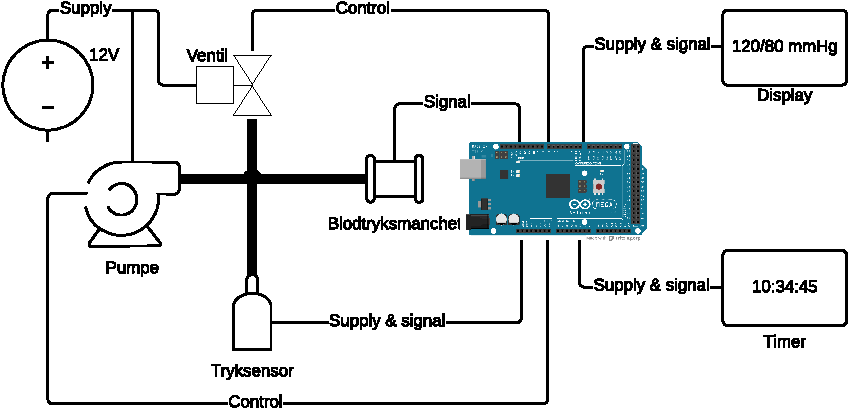
\includegraphics[width = \textwidth]{billeder/systemDrawing-crop.pdf}
	\caption{Oversigt over \textit{Konditioneringsapparatet}} \label{fig:systemTegning}
\end{figure}

Alle funktioner kræver at manchetten monteres på enten armen eller benet. Ved konditioneringsbehandling måles blodtrykket og der afklemmes ved et tryk svarende til 25mmHg højere end det målte systoliske tryk. Dernæst udføres konditioneringsbehandling. Systemet logger information omkring konditioneringsbehandling. Okklusionstræning udføres ved at pumpe manchettrykken op til 100 mmHg og holde det trykket indtil brugeren stopper forløbet. 

Endvidere kan \textit{konditioneringsapparatet} konfigureres gennem ændring af variablerne antal cyklusser og tid pr cyklus.


\section{Brugergrænseflade}
\textit{Konditioneringsapparatets} brugergrænseflade består af 2 knapper og en skærm. Desuden findes en \textit{modeswitch} på prototypen, en knap med 3 stadier, som styre om apparatet skal konditionerer, okklusionstræne eller konfigureres.  

\section{Data logging}
Systemet gemmer information omkring konditioneringsbehandling. Disse gemmes på et SD kort, for at sikre dokumentation af konditioneringsbehandling.

\begin{figure}[H]
	\centering
	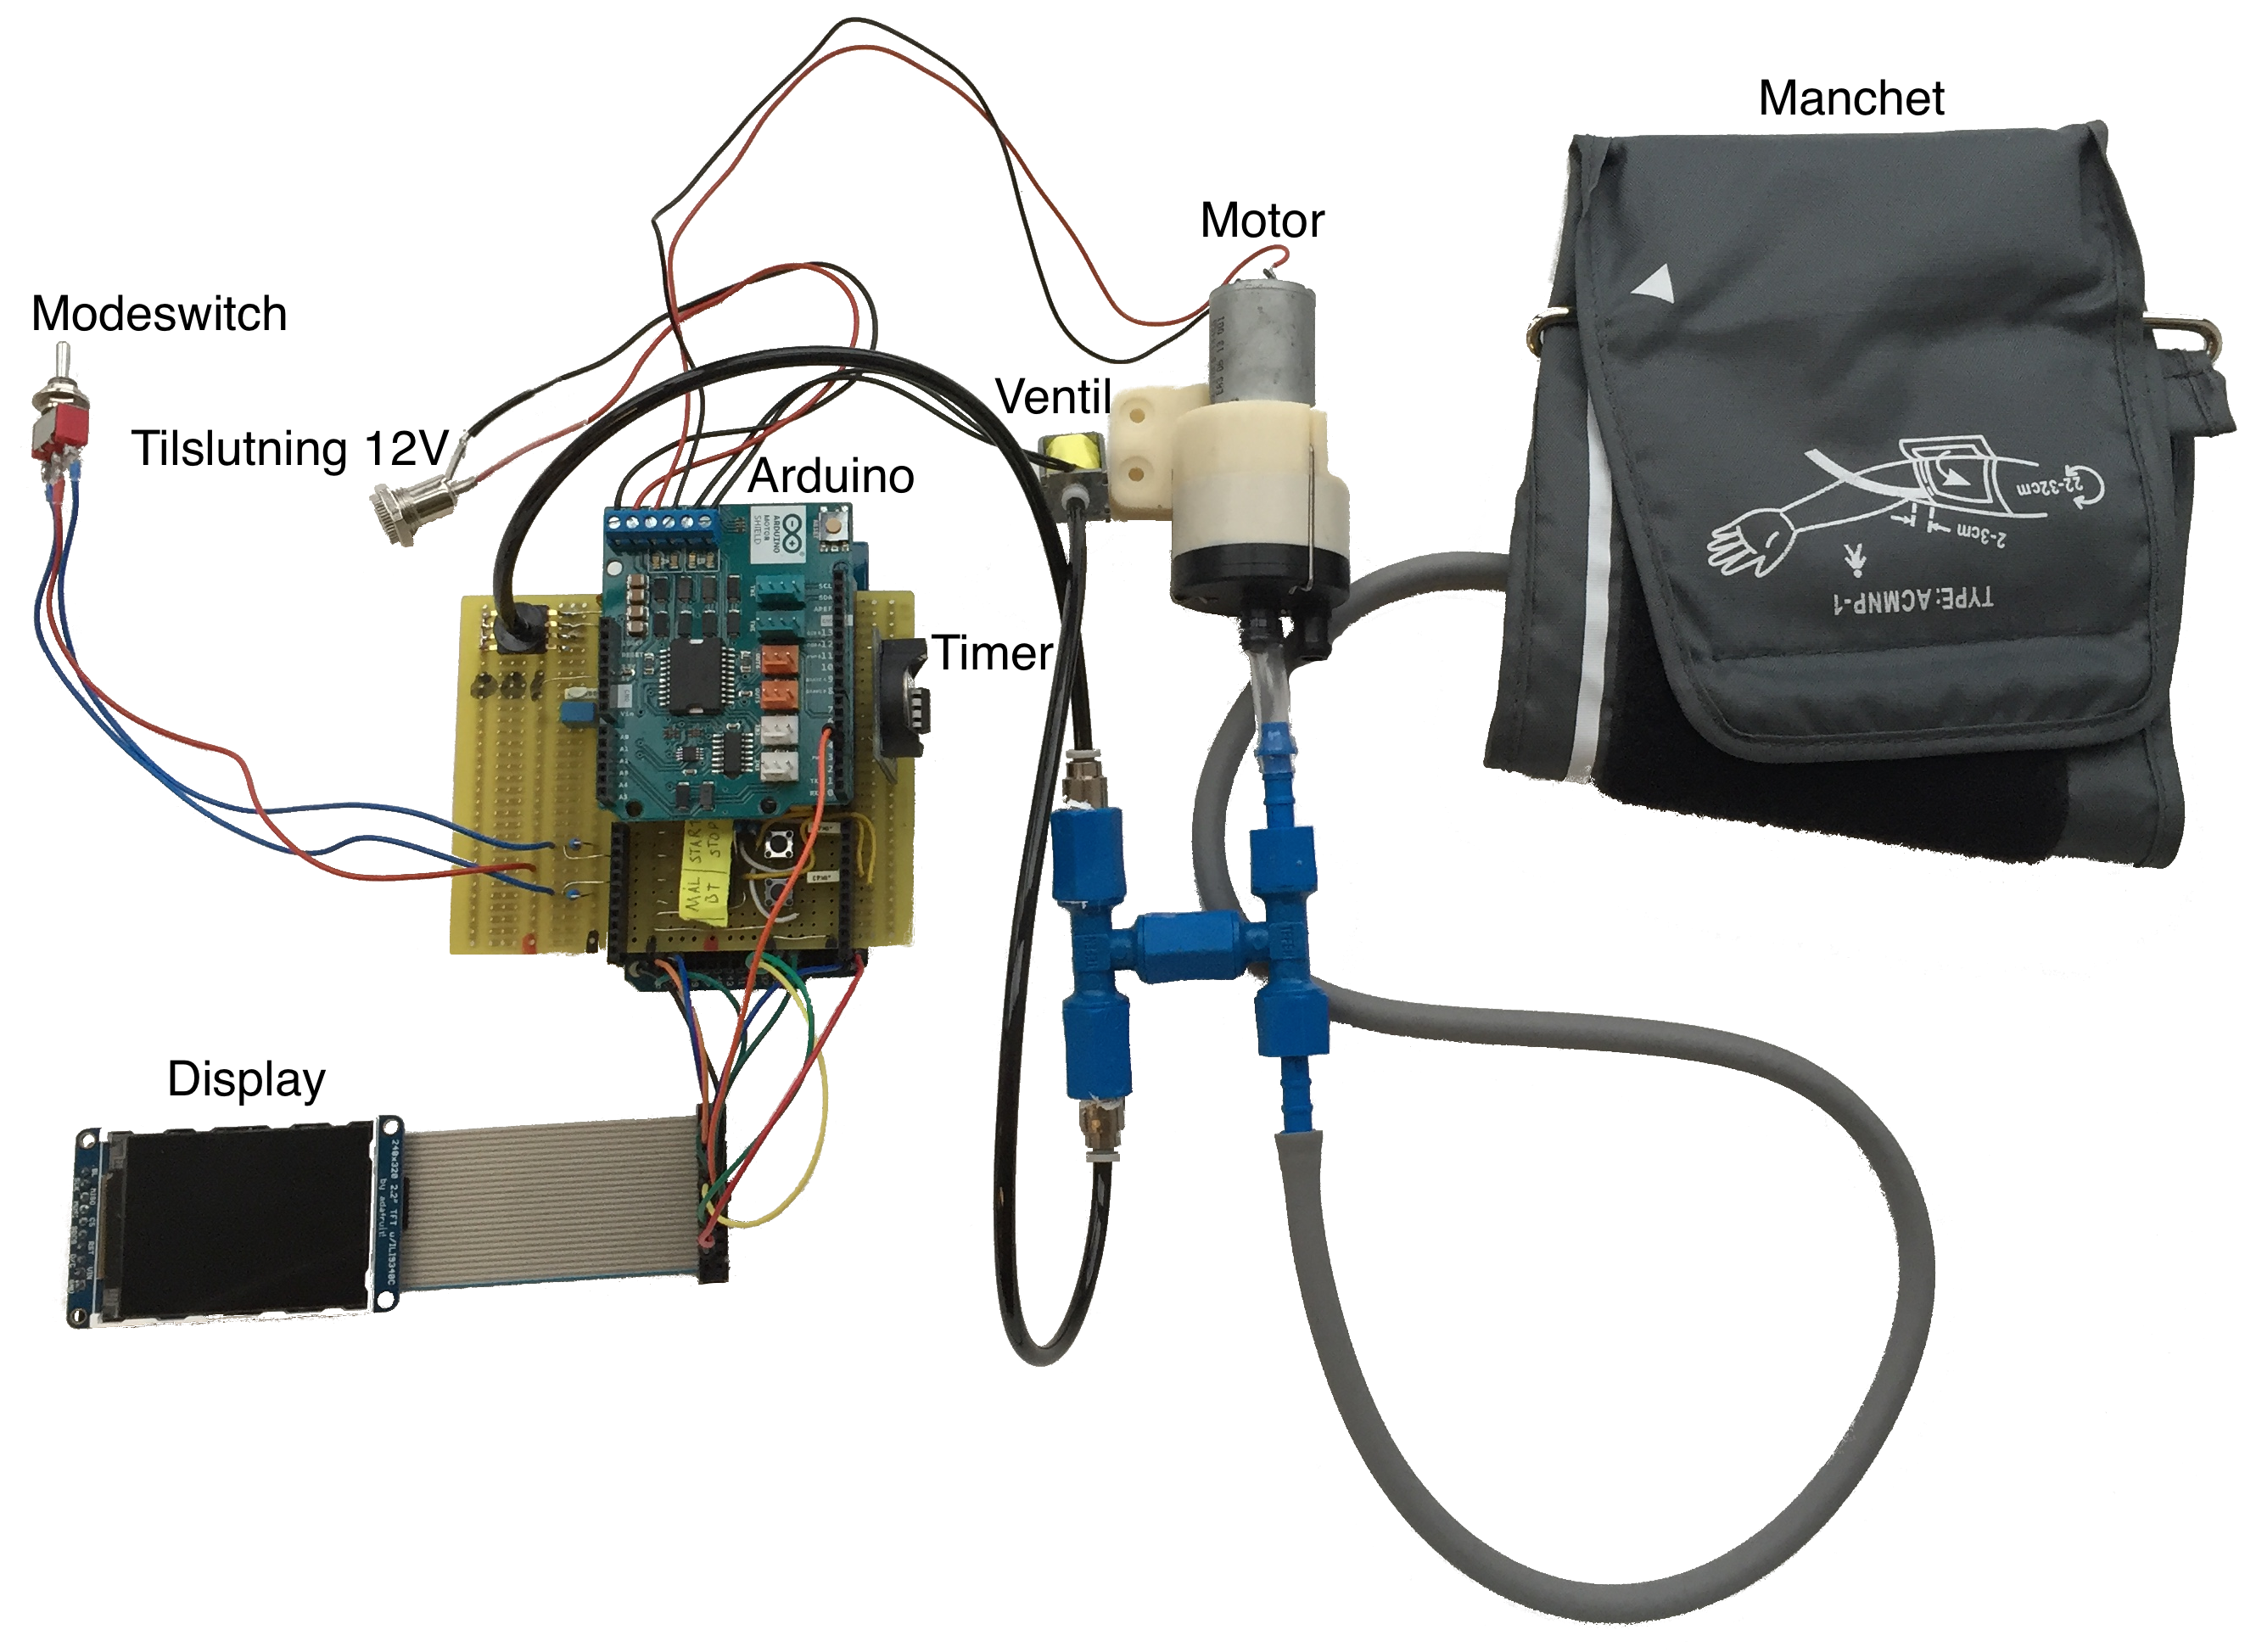
\includegraphics[width = \textwidth]{billeder/Konditioneringsapparat-tekst.png}
	\caption{Billede af \textit{Konditioneringsapparatet}} \label{fig:oversigtsbillede}
\end{figure}